\documentclass[12pt]{article}

\usepackage[margin=0.5in]{geometry}

\usepackage{hyperref}
\hypersetup{
    colorlinks=true,
    linkcolor=blue,
    filecolor=magenta,      
    urlcolor=blue,
}
 
\urlstyle{same}

\usepackage{datetime}
\newdateformat{specialdate}{\twodigit{\THEDAY}.\twodigit{\THEMONTH}.\THEYEAR}

\usepackage{polski}
\usepackage[polish]{babel}
\usepackage[utf8]{inputenc}

\usepackage{titling}

\usepackage{framed}
\usepackage[svgnames]{xcolor}
\colorlet{shadecolor}{Gainsboro!50}

\usepackage{float}
\usepackage{graphicx}
\graphicspath{ {./images/} }

\usepackage{verbatim}

\usepackage{caption}
\captionsetup[figure]{name=Fig.}

\title{Clustering of sequences}
\author{Maciej Sikora}
\date{\specialdate\today}


\begin{document}
\maketitle

\section{Dane do klastrowania}
Dane pochodzą z bazy Pfam przez pobranie sekwencji seedu dla losowych rodzin.
Wybrane rodziny musiały mieć co najmniej 10 sekwencji, a w przypadku liczby sekwencji większej niż 30 - liczba ta została zredukowana do 30.

\section{Metody klastrowania}
Klastrowanie zostało wykonane dwoma metodami:
\begin{itemize}
\item cd-hit
\item CLANS
\end{itemize}
Klastrowanie cd-hit zostało wykonane z parametrem podobieństwa 40\% dla porównywania słów długości 2 (-c 0.4 -n 2)

Klastrowanie CLANS opiera się na algorytmie BlastP na podstawie którego liczone są wartości attraction value z zakresu 0 -- 1, gdzie 1 oznacza najbardziej podobne sekwencje. Dalej sekwencje są optymalizowane pod względem attraction value na przestrzeni 2-wymiarowej. Dalej klastry wyznaczane są na podstawie połączeń tak, że najmniejszy klaster może mieć 10 sekwencji.

\section{Wyniki i analiza}
Jakość klastrowania została wyznaczona przez liczenie wartości indexu Jaccard all vs all w sposób binarny.
Dla każdej ze 100 rodzin (true label) zapisany został najlepszy wynik indeksu i sporządzony histogram wartości.

\subsection{cd-hit}
W tym przypadku cd-hit zwrócił 874 klastry - można więc się spodziewać, że niskie wyniki będą w dużym stopniu wynikały z niekompletności predykcji klastrów.
Ok. 15 klastrów posiadało wartości indeksu powyżej 0.9.
\begin{figure}[H]
\begin{center}
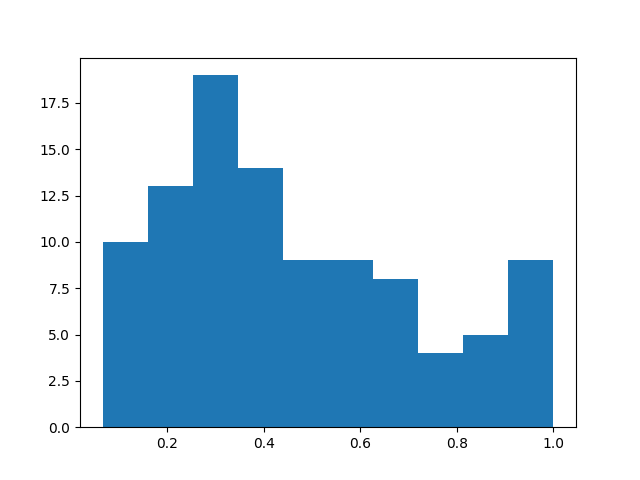
\includegraphics[width=0.7\textwidth]{myplot_cdhit}
\end{center}
\end{figure}


\subsection{CLANS}
CLANS zwrócił 75 klastrów - tu niskie wartości mogą więc wynikać z faktu, że 2 rodziny zostały zaklasyfikowane jako jedna (prawdopodobnie pochodzą z jednego klanu) -- potwierdza to fakt, że wiele klastrów ma rozmiar 60, a około 25 klastrów ma wartość 0.
Klastrowanie wygląda jednak znacznie lepiej w tym przypadku.

\begin{figure}[H]
\begin{center}
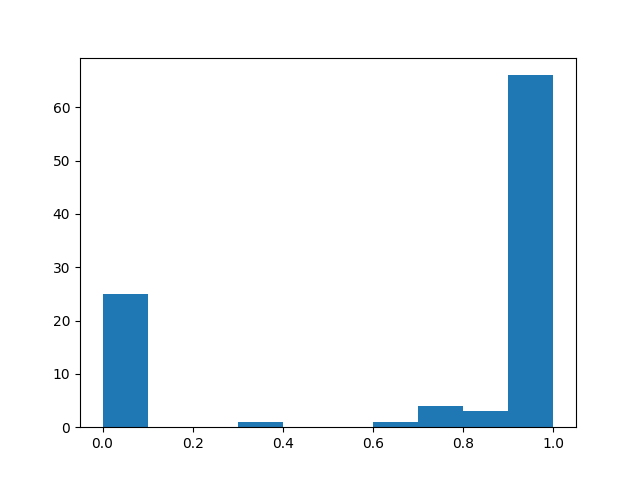
\includegraphics[width=0.7\textwidth]{myplot}
\end{center}
\end{figure}

\subsection{CLANS dla podziału na klany}
W celu zweryfikowania hipotezy dla klastrowania dla klanów przeprowadzone zostało dodatkowe liczenie histogramu.
Przy podziale na klany mamy 93 grupy (klany lub rodziny dla nieposiadających klanu). Liczba grup z wartością indeksu 0 nieco spadła, co może potwierdzać hipotezę.

\begin{figure}[H]
\begin{center}
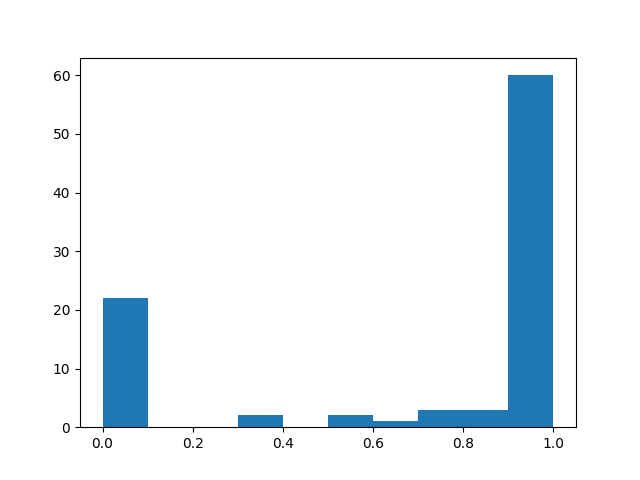
\includegraphics[width=0.7\textwidth]{myplot_klany}
\end{center}
\end{figure}

\end{document}

\begin{comment}
BEGIN EXAMPLE PARAGRAPH:

-----Kod w szarym boxie-----
\begin{shaded}\small
\begin{alltt}
KOD
\end{alltt}
\end{shaded}

-----Wstawianie obrazka-----
\begin{figure}[H]
\begin{center}
\includegraphics[width=\textwidth]{raw_url_fasta}
\caption{Przykład umiejscowienia sekwencji przy użyciu surowego linku.}
\end{center}
\end{figure}

-----Tabela-----
\begin{center}
\begin{tabular}{ | l | l | } 
\hline
Nazwa & Dodatek do linku\\ 
\hline
\hline
AC & id\\
\hline
Entry name & entry\%20name\\ 
\hline
Czy Reviewed & reviewed\\ 
\hline
Referencje do Pfam & database(Pfam)\\ 
\hline
Sekwencja & sequence\\ 
\hline
\end{tabular}
\end{center}

\end{comment}